%!Tex root=../report.tex

\section{Background}
We seek to investigate the performance of various tree policies in Monte Carlo Tree Search with application to POMDP problems. In this section, we give a general overview of the two domains.

\subsection{Monte Carlo Tree Search}
Monte Carlo Tree Search (MCTS) is a heuristic algorithm that is used for on-line planning. At each step, it recursively generates a search tree of rewards for all available actions (and subsequent actions) by repeatedly sampling a random path of actions from the current state. The reward of an action is computed as the aggregate reward over all paths that follow this action, up to a fixed search depth (100 in this paper). Through this approach, it effectively samples the probability distribution over rewards given actions by investigating arbitrary (long-term) consequences of these actions.

Consider by means of example a game of chess: the ultimate goal of a player is to capture the opponent's king while keeping their own king safe. In order to obtain this goal a (possibly large) number of moves have to be made by both players alternatingly. Deciding which move to make at every step, given the state of the game, is key to winning the game. These moves can have both direct rewards (like the capture of an opponents piece), but will generally only have effect a number of turns after the move was made, and this effect may continue to have implications throughout the rest of the game. As such, the number of possible states in a game of chess is enormous and it is unfeasible to compute the ultimate reward of every sequence of actions.

MCTS solves this problem by only evaluating a select number of action sequences and possible responses, and finally selecting the move with the highest aggregated reward, because this move is most likely to generate a high reward (taking into account possible counter-moves). To achieve this, MCTS constructs a tree that models the game, as summarized in \Cref{alg:mcts}. MCTS constructs the tree by iteratively executing UCTSearch (as first proposed by Kocsis \etal \cite{kocsis2006bandit}), which in turn determines the path to be simulated and updates the tree nodes with their expected rewards. Every action (node) results in an immediate reward $r$ and a relayed reward $delayedr$, which is a result of later chosen actions. The tree is constructed by sampling different combinations of actions (paths through the tree). When either a leaf node or the search horizon is reached, a reward is obtained which is then propagated back to the root. 

Notice that there are two black box operations present: TreePolicy and SIMLULATE. TreePolicy is an algorithm that decides which node should be visited next, which will be more thoroughly explained in Section \ref{sec:tp}. SIMULATE is a domain dependent operation, that simulates the effects of choosing $v$ as the next action; it returns both an immediate reward for playing that action and relays whether this action sequence leads to an end state.

\begin{algorithm}
\begin{algorithmic}[1]
\Function{MCTS}{$s_0$, $sims$}
\State create root node $v_0$ with state $s_0$
\For{$i := 0 \to sims$} \do \\ \\
~~~~~~~~	UCTSearch($v_i$)
~~~~~~~~	\State \Return best\_child($v_0$)
\EndFor \\
\EndFunction

\Function{UCTSearch}{$v$}
	\State create simulation tree with root node $v_0$ and state $s_0$
	\State $v := $ TreePolicy($v$)
	\State $\{r$, terminated$\}$ := SIMULATE($v$)
	\If{!terminated}\State $delayedr :=$ UCTSearch($v$) 
	\Else \State $delayedr := 0$
	\EndIf
	\State $v$.visits++, $v$.totalReward += $ r + delayedr$ 
	\State \Return $v$.totalReward/$v$.visits
\EndFunction
\end{algorithmic}
\caption{The MCTS Algorithm}
\label{alg:mcts}
\end{algorithm}

\subsection{Partially Observable Monte-Carlo Planning}
In many practical problems, the true state of the entire world is not known; instead, a belief may exist regarding the state of other positions, which can be updated with each new observation. Planning problems in which the environment is only partially observable are called POMDPs. These environments pose a challenge for search algorithms: at each point in time an action must be selected of which the long-term consequences are ever less certain. Silver \& Veness observe that Monte-Carlo search trees are well-suited to deal with this uncertainty and propose to extend MCST algorithms with a belief-state filter to apply these to POMDPs (naming the new algorithm POMCP) \cite{silver2010monte}. The motivation is that the Monte-Carlo process effectively simulates probability distributions over potential rewards, removing the problem of explicitly factorizing the true distributions. Indeed, Silver \& Veness find that MCTS yields superior performance to previous approaches on three games with various state-space sizes and dynamics. The POMCP algorithm, with a description of its process, is illustrated in \Cref{fig:pomcp} (retrieved from \cite{silver2010monte}). 

\begin{figure*}[ht!]
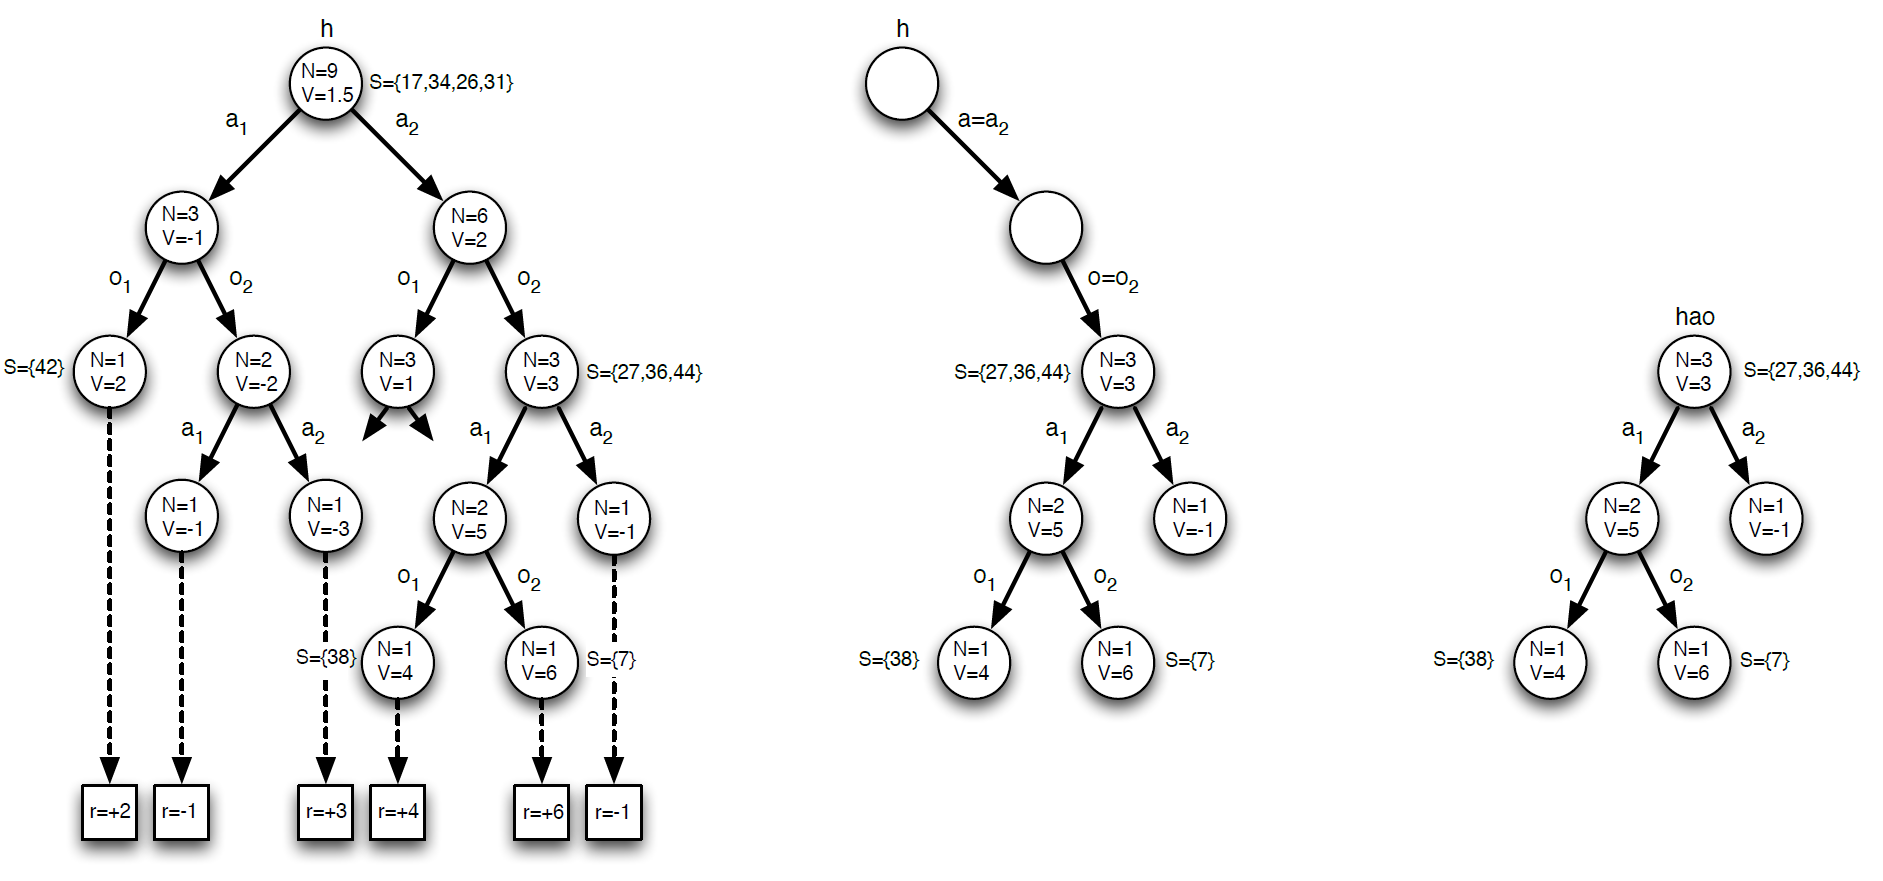
\includegraphics[width=\linewidth]{pomdp.png}
\caption{An illustration of the three steps in a single step of the POMCP process, from \cite{silver2010monte}. Each step in the tree consists of an action and corresponding observation. The algorithm first simulates a large number of actions and potential observations (left), then aggregates the rewards and chooses the action with the highest mean return (middle) to which it receives the true observation. Finally, the believe-state is updated and the tree is pruned, the process starts again from the new state (right).}
\label{fig:pomcp}
\end{figure*}
